%%%%%%%%%%%%%%%%%%%%%%%%%%%%%%%%%%%%%%%%%
% Beamer Presentation
% LaTeX Template
% Version 1.0 (10/11/12)
%
% This template has been downloaded from:
% http://www.LaTeXTemplates.com
%
% License:
% CC BY-NC-SA 3.0 (http://creativecommons.org/licenses/by-nc-sa/3.0/)
%
%%%%%%%%%%%%%%%%%%%%%%%%%%%%%%%%%%%%%%%%%

%----------------------------------------------------------------------------------------
%	PACKAGES AND THEMES
%----------------------------------------------------------------------------------------

\documentclass{beamer}
\usepackage{xcolor}
\usepackage{graphicx}
\usepackage{tikz}
\usepackage{listings}
\usepackage{multicol}
\usepackage[autoload=false]{jlcode}

\DeclareMathOperator{\diag}{diag}

\definecolor{applegreen}{rgb}{0.55, 0.71, 0.0}
\definecolor{blue(ncs)}{rgb}{0.0, 0.45, 0.60}
\definecolor{burgundy}{rgb}{0.5, 0.0, 0.13}

\definecolor{cadet}{rgb}{0.33, 0.41, 0.47}
\definecolor{airforceblue}{rgb}{0.36, 0.54, 0.66}

\lstdefinestyle{C}{
  language=C,
  emptylines=1,
  breaklines=true,
  basicstyle=\ttfamily\color{black},
  identifierstyle=\ttfamily,
  keywordstyle=\color[rgb]{0.0, 0.0, 1.0},
  stringstyle=\color[rgb]{1.0, 0.0, 0.0},
  commentstyle=\color{gray}\slshape,
}

\lstdefinestyle{assembly}{
  emptylines=1,
  breaklines=true,
  basicstyle=\ttfamily\color{black},
  identifierstyle=\ttfamily,
  keywordstyle=\color[rgb]{1.0, 0.0, 1.0},
  stringstyle=\color[rgb]{1.0, 0.0, 0.0},
  commentstyle=\color{gray}\slshape,
  morekeywords={vmovapd, vfmadd231pd,vfnmadd213pd, vmulpd},
}

\mode<presentation> {

\usetheme{CambridgeUS}

\usecolortheme{wolverine}

\definecolor{gold}{HTML}{D4A017}
\definecolor{darkgold}{HTML}{B7950B}

\setbeamercolor{palette primary}{bg=cadet,fg=white}
\setbeamercolor{palette secondary}{bg=airforceblue,fg=white}
\setbeamercolor{palette tertiary}{bg=black,fg=white}
\setbeamercolor{palette quaternary}{bg=cadet,fg=white}

\setbeamercolor{frametitle}{bg=airforceblue,fg=white}

\setbeamercolor{section number projected}{bg=black,fg=cadet}
\setbeamercolor{item}{fg=black,bg=cadet}

\setbeamertemplate{page number in head/foot}[framenumber]
}

\usepackage{graphicx} % Allows including images
\usepackage{booktabs} % Allows the use of \toprule, \midrule and \bottomrule in tables

%----------------------------------------------------------------------------------------
%	TITLE PAGE
%----------------------------------------------------------------------------------------

\title[LFA of High-Order Matrix-Free FEM]{Local Fourier Analysis of Domain Decomposition and Multigrid Methods for High-Order Matrix-Free Finite Elements} % The short title appears at the bottom of every slide, the full title is only on the title page

\author{Jeremy L Thompson} % Your name
\institute[CU Boulder] % Your institution as it will appear on the bottom of every slide, may be shorthand to save space
{University of Colorado Boulder \\ % Your institution for the title page
\medskip
\textit{jeremy@jeremylt.org} % Your email address
}
\date{July 8, 2021} % Date, can be changed to a custom date

\begin{document}

\begin{frame}
\titlepage % Print the title page as the first slide
\end{frame}

%------------------------------------------------

\begin{frame}
\begin{center}
\frametitle{Funding}

This work is supported by the Exascale Computing Project (17-SC-20-SC), a collaborative effort of two U.S. Department of Energy organizations (Office of Science and the National Nuclear Security Administration) responsible for the planning and preparation of a capable exascale ecosystem, including software, applications, hardware, advanced system engineering and early testbed platforms, in support of the nation’s exascale computing imperative.

\end{center}
\end{frame}
 
%------------------------------------------------

\begin{frame}
\frametitle{Overview} % Table of contents slide, comment this block out to remove it
\tableofcontents % Throughout your presentation, if you choose to use \section{} and \subsection{} commands, these will automatically be printed on this slide as an overview of your presentation
\end{frame}

%----------------------------------------------------------------------------------------
%	PRESENTATION SLIDES
%----------------------------------------------------------------------------------------

%------------------------------------------------
\section{Introduction}
%------------------------------------------------

\begin{frame}
\begin{center}
\frametitle{Big Picture}

\begin{itemize}

\item High-order matrix-free representations of PDEs are better suited to modern hardware than sparse matrices\\

~\\

\item High-order matrix-free representations require preconditioned\\iterative solvers\\

~\\

\item Local Fourier Analysis (LFA) provides sharp convergence estimates\\for these preconditioners\\

~\\

\item We develop LFA of p-multigrid and Balancing Domain Decomposition by Constraints (BDDC) on high-order element subdomains\\

~\\

\item Further, we investigate LFA of p-multigrid with a BDDC smoother

\end{itemize}

\end{center}
\end{frame}

%------------------------------------------------

\begin{frame}
\begin{center}
\frametitle{Reproducibility}

Transparency and reproducibility are the lifeblood of scientific advancement\\

~\\

All software and data used in this dissertation is all open source\\

~\\

\begin{itemize}

\item \href{https://www.github.com/jeremylt/LFAToolkit.jl}{https://www.github.com/jeremylt/LFAToolkit.jl}\\

~\\

\item \href{https://www.github.com/CEED/libCEED}{https://www.github.com/CEED/libCEED}\\

~\\

\item \href{https://www.mcs.anl.gov/petsc}{https://www.mcs.anl.gov/petsc}\\

~\\

\item \href{https://github.com/jeremylt/dissertation}{https://github.com/jeremylt/dissertation}\\

\end{itemize}

\end{center}
\end{frame}

%------------------------------------------------
\section{High-Order Matrix-Free FEM}
%------------------------------------------------

\begin{frame}
\begin{center}
\frametitle{Modern Hardware}

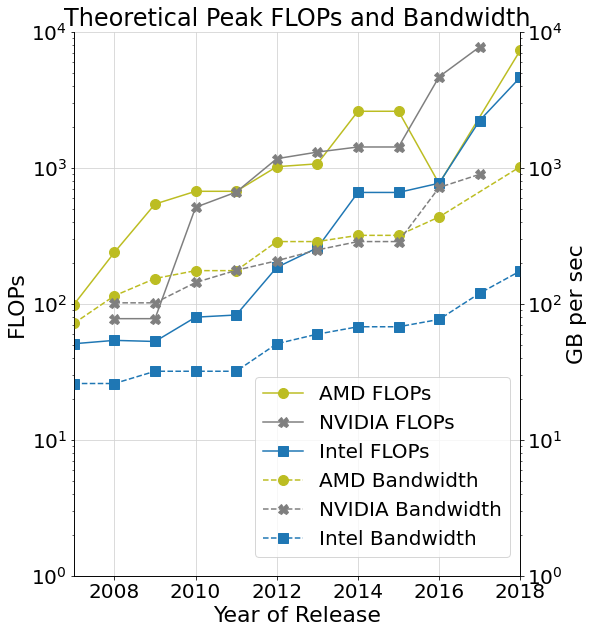
\includegraphics[height=5.5cm]{../img/peakFlopsAndBandwidth_tall}
\hspace{1cm}
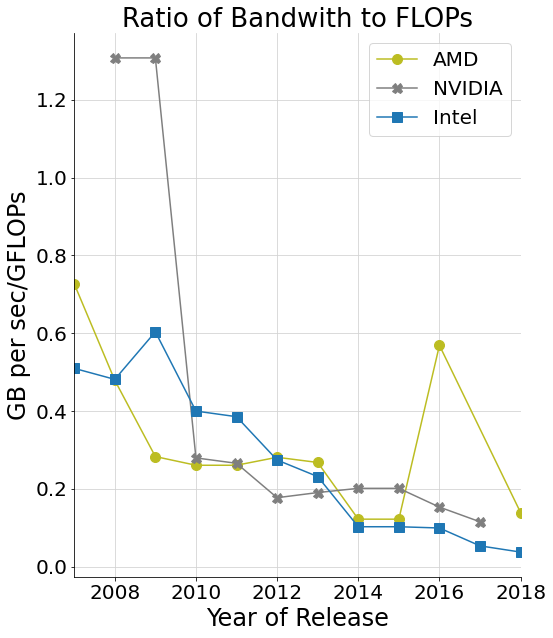
\includegraphics[height=5.5cm]{../img/peakRatio_tall}

Modern hardware has lower memory bandwidth than FLOPs \cite{kruppcomparison}

\end{center}
\end{frame}

%------------------------------------------------

\begin{frame}
\begin{center}
\frametitle{Benefits of Matrix-Free}

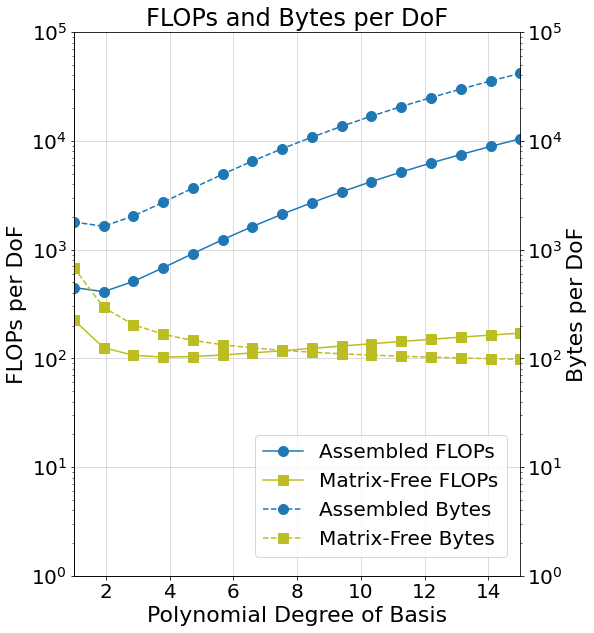
\includegraphics[height=5.5cm]{../img/assembledVsMatrixFree_tall}
\hspace{1cm}
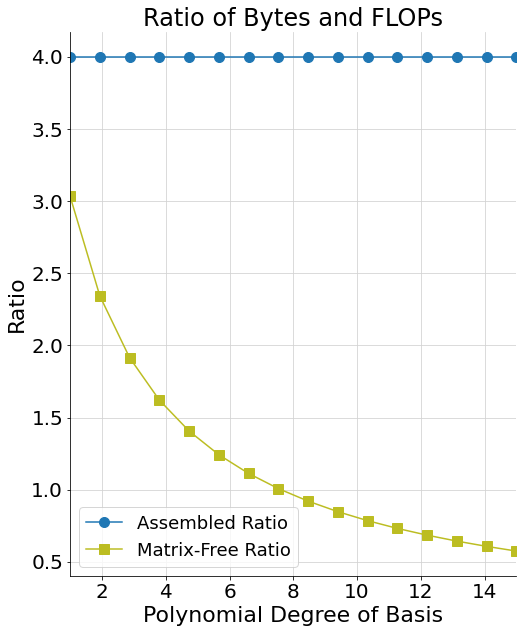
\includegraphics[height=5.5cm]{../img/assembledVsMatrixFreeBalance_tall}

{\small Requirements for matrix-vector product with sparse matrix vs matrix-free\\ for screened Poisson $\nabla^2 u - \alpha^2 u = f$ in 3D}\\

{\bf Matrix-free representations using tensor product bases better match modern hardware limitations}

\end{center}
\end{frame}

%------------------------------------------------

\begin{frame}
\begin{center}
\frametitle{Matrix-Free Representation}

Weak form for an arbitrary second order PDE \cite{brown2010efficient}:\\

\begin{equation}
\begin{array}{c}
\text{find } u \in V \text{ such that for all } v \in V\\
\langle v, u \rangle = \int_{\Omega} v \cdot f_0 \left( u, \nabla u \right) + \nabla v : f_1 \left( u, \nabla u \right) = 0
\end{array}
\label{eq:weak_form}
\end{equation}

\begin{itemize}

\item $\cdot$ - contraction over fields\\

\item $:$ - contraction over fields and spatial dimensions\\

\end{itemize}

\end{center}
\end{frame}

%------------------------------------------------

\begin{frame}
\begin{center}
\frametitle{Matrix-Free Representation}

Galerkin form for an arbitrary second order PDE:\\

\begin{equation}
\sum_e \mathcal{E}^T \left[ \left( {\color{blue(ncs)}\mathbf{N}}^e \right)^T {\color{applegreen}\mathbf{W}}^e \Lambda \left( {\color{applegreen}f_0} \left( u^e, \nabla u^e \right) \right) + \sum_{i = 0}^{d - 1} \left( {\color{blue(ncs)}\mathbf{D}}_i^e \right)^T {\color{applegreen}\mathbf{W}}^e \Lambda \left( {\color{applegreen}f_1} \left( u^e, \nabla u^e \right) \right) \right] = 0
\label{eq:galerkin_form}
\end{equation}

\begin{itemize}

\item $\mathcal{E}$ - element assembly/restriction operator\\

\item ${\color{blue(ncs)}\mathbf{N}}^e$ - interpolation to quadrature points\\

\item ${\color{blue(ncs)}\mathbf{D}}_i^e$ - derivatives at quadrature points\\

\item ${\color{applegreen}\mathbf{W}}^e$ - quadrature weights\\

\item $\Lambda$ - pointwise multiplication at quadrature points\\

\end{itemize}

\end{center}
\end{frame}

%------------------------------------------------

\begin{frame}
\begin{center}
\frametitle{libCEED Representation}

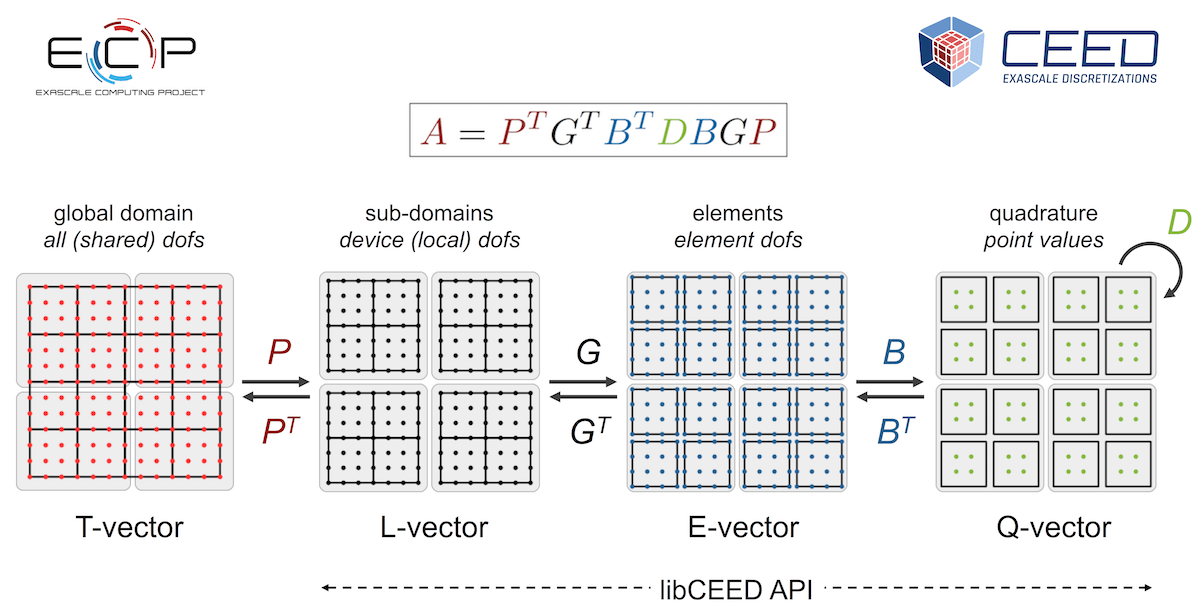
\includegraphics[height=4.5cm]{../img/libCEEDAPI}\cite{libceed-user-manual}

\begin{itemize}

\item ${\color{burgundy}\mathbf{P}}$ - parallel element assembly operator

\item $\mathbf{G}$ - local element assembly operator\\

\item ${\color{blue(ncs)}\mathbf{B}}$ - basis action operator\\

\item ${\color{applegreen}\mathbf{D}}$ - weak form and geometry at quadrature points\\

\end{itemize}

\end{center}
\end{frame}

%------------------------------------------------
\section{LFA of High-Order FEM}
%------------------------------------------------

\begin{frame}
\begin{center}
\frametitle{LFA Background}

Consider a scalar Toeplitz operator $L_h$ on the infinite 1D grid $G_h$

\begin{equation}
\begin{gathered}
L_h \mathrel{\hat{=}} \left[ s_\kappa \right]_h \left( \kappa \in V \right)\\
L_h w_h \left( x \right) = \sum_{\kappa \in V} s_\kappa w_h \left( x + \kappa h \right)
\end{gathered}
\end{equation}

\begin{flushleft}
where
\end{flushleft}

\begin{itemize}

\item $V \subset \mathcal{Z}$ is an index set

\item $s_k \in \mathcal{R}$ are constant coefficients

\item $w_h \left( x \right)$ is a $l^2$ function on $G_h$

\end{itemize}

\end{center}
\end{frame}

%------------------------------------------------

\begin{frame}
\begin{center}
\frametitle{LFA Background}

If for all grid functions $\varphi \left( \theta, x \right)$

\begin{equation}
L_h \varphi \left( \theta, x \right) = \tilde{L}_h \left( \theta \right) \varphi \left( \theta, x \right)
\end{equation}

~\\

then $\tilde{L}_h \left( \theta \right) = \sum_{\kappa \in V} s_\kappa e^{\imath \theta \kappa}$ is the {\bf symbol} of $L_h$\\

~\\

Our function can be diagonalized by the standard Fourier modes

\end{center}
\end{frame}

%------------------------------------------------

\begin{frame}
\begin{center}
\frametitle{LFA Background}

For a $q \times q$ system of equations, the matrix symbol is given by

\begin{equation}
\mathbf{L}_h =
\begin{bmatrix}
    L_h^{1, 1} && \cdots && L_h^{1, q}        \\
    \vdots               && \vdots && \vdots  \\
    L_h^{q, 1} && \cdots && L_h^{q, q}        \\
\end{bmatrix}
\hspace{0.5cm}
\Rightarrow
\hspace{0.5cm}
\tilde{\mathbf{L}}_h =
\begin{bmatrix}
    \tilde{L}_h^{1, 1} && \cdots && \tilde{L}_h^{1, q}  \\
    \vdots             && \vdots && \vdots              \\
    \tilde{L}_h^{q, 1} && \cdots && \tilde{L}_h^{q, q}  \\
\end{bmatrix}
\end{equation}

\end{center}
\end{frame}

%------------------------------------------------

\begin{frame}
\begin{center}
\frametitle{LFA of High-Order FEM}

For a scalar PDE operator on a single 1D finite element

\begin{equation}
\tilde{{\color{burgundy}\mathbf{A}}} \left( \boldsymbol{\theta} \right) = \mathbf{Q}^T \left( {\color{burgundy}\mathbf{A}}^e \odot \left[ e^{\imath \left( \mathbf{x}_j - \mathbf{x}_i \right) \cdot \boldsymbol{\theta} / \mathbf{h}} \right] \right) \mathbf{Q}
\label{eq:symbolhighorder}
\end{equation}

\begin{flushleft}
where
\end{flushleft}

\begin{equation}
{\color{burgundy}\mathbf{A}}^e = {\color{blue(ncs)}\mathbf{B}}^T {\color{applegreen}\mathbf{D}} {\color{blue(ncs)}\mathbf{B}}
\label{eq:localoperator}
\end{equation}

\begin{equation}
\mathbf{Q} =
\begin{bmatrix}
    \mathbf{I}   \\
    \mathbf{e}_0 \\
\end{bmatrix} =
\begin{bmatrix}
    1      && 0      && \cdots && 0      \\
    0      && 1      && \cdots && 0      \\
    \vdots && \vdots && \vdots && \vdots \\
    0      && 0      && \cdots && 1      \\
    1      && 0      && \cdots && 0      \\
\end{bmatrix}
\label{eq:fouriermodelocalization1d}
\end{equation}

\end{center}
\end{frame}

%------------------------------------------------

\begin{frame}
\begin{center}
\frametitle{LFA of High-Order FEM}

Symbol naturally extends to multiple components and higher dimensions\\

~\\

\begin{columns}[onlytextwidth]
  \begin{column}{0.45\textwidth}
    \begin{center}
    Multiple Components:
    \end{center}
    \begin{equation}
    \mathbf{Q}_n = \mathbf{I}_n \otimes \mathbf{Q}
    \end{equation}
  \end{column}

  \begin{column}{0.45\textwidth}
    \begin{center}
    Multiple Dimensions:
    \end{center}
    \begin{equation}
    \mathbf{Q}_{nd} = \mathbf{Q} \otimes \mathbf{Q} \otimes \dots \otimes \mathbf{Q}
    \end{equation}
  \end{column}
\end{columns}

\end{center}
\end{frame}

%------------------------------------------------

\begin{frame}[fragile]
\begin{center}
\frametitle{Example: Scalar Poisson}

\begin{equation}
  \int \nabla v \nabla u = \int f v
\end{equation}

\begin{itemize}

\item ${\color{blue(ncs)}\mathbf{B}}$ - given by tensor H1 Lagrange basis\\

\item ${\color{applegreen}\mathbf{D}}$ - given by quadrature weights and product\\

\end{itemize}

{\small
\begin{jllisting}[language=julia, style=jlcodestyle]
# mesh
dim = 1
mesh = Mesh1D(1.0)

# basis
p = 3
ncomp = 1
basis = TensorH1LagrangeBasis(p+1, p+1, ncomp, dim)

# weak form
function diffusionweakform(du::Array{Float64}, w::Array{Float64})
    return dv = du*w[1]
end
\end{jllisting}
}

\end{center}
\end{frame}

%------------------------------------------------

\begin{frame}
\begin{center}
\frametitle{Example: Scalar Poisson}

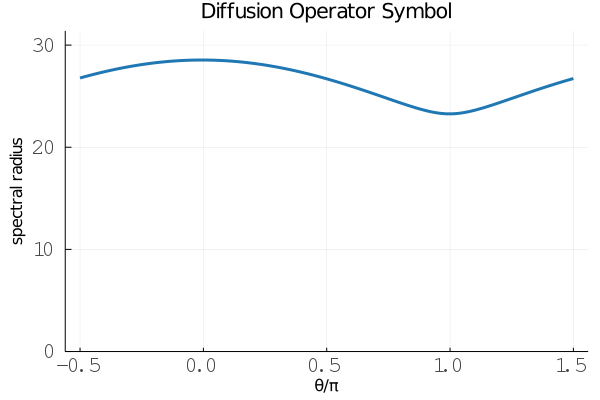
\includegraphics[height=3.9cm]{../img/diffusionSymbol1D}
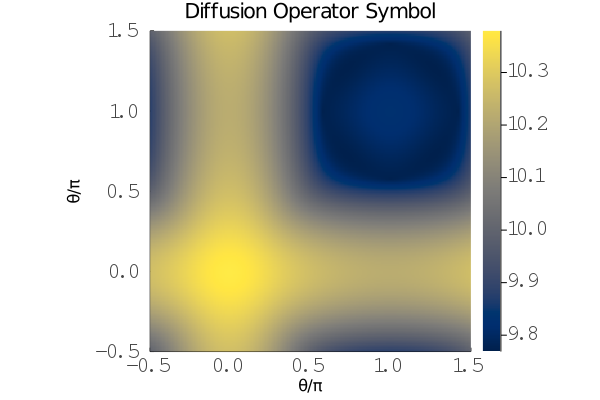
\includegraphics[height=3.9cm]{../img/diffusionSymbol2D}

Scalar Poisson problem on quartic elements\\

~\\

low frequencies - $\theta \in T^{\text{low}} = \left[ - \pi / 2, \pi / 2 \right)^d$\\

high frequencies - $\theta \in T^{\text{high}} = \left[ - \pi / 2, 3 \pi / 2 \right)^d \setminus T^{\text{low}}$

\end{center}
\end{frame}

%------------------------------------------------

\begin{frame}
\begin{center}
\frametitle{LFA of High-Order Smoothers}

Error propagation operator for smoothers given by

\begin{equation}
\mathbf{S} = \mathbf{I} - \mathbf{M}^{-1} {\color{burgundy}A}
\end{equation}

with a symbol given by

\begin{equation}
\tilde{\mathbf{S}} \left( \omega, \boldsymbol{\theta} \right) = \mathbf{I} - \tilde{\mathbf{M}}^{-1} \left( \omega, \boldsymbol{\theta} \right) \tilde{{\color{burgundy}A}} \left( \boldsymbol{\theta} \right)
\end{equation}

\end{center}
\end{frame}

%------------------------------------------------

\begin{frame}
\begin{center}
\frametitle{Jacobi Smoothing}

Jacobi smoothing given by

\begin{equation}
\mathbf{M}^{-1} = \omega \hspace{1mm} \diag \left( {\color{burgundy}A} \right)^{-1}
\end{equation}

with an error symbol given by

\begin{equation}
\tilde{\mathbf{S}} \left( \omega, \boldsymbol{\theta} \right) = \mathbf{I} - \omega \hspace{1mm} \left( \mathbf{Q}^T \diag \left( {\color{burgundy}A}^e \right) \mathbf{Q} \right)^{-1} \tilde{{\color{burgundy}A}} \left( \boldsymbol{\theta} \right)
\end{equation}

\end{center}
\end{frame}

%------------------------------------------------

\begin{frame}
\begin{center}
\frametitle{Example: Jacobi Smoothing}

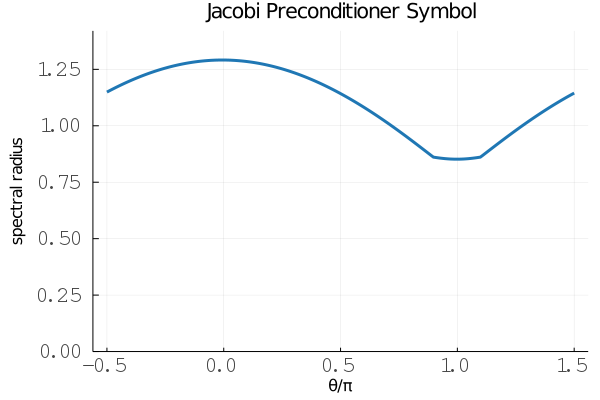
\includegraphics[height=3.9cm]{../img/JacobiSymbol1D}
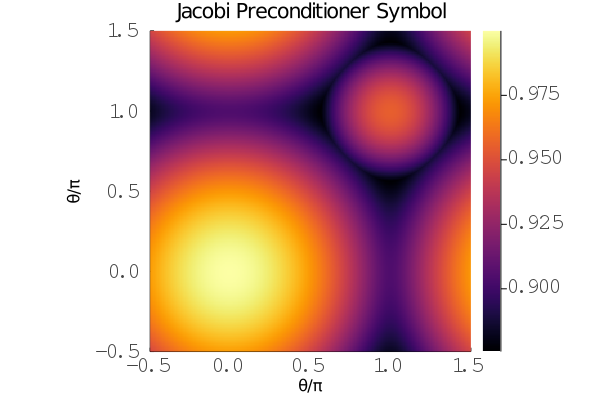
\includegraphics[height=3.9cm]{../img/JacobiSymbol2D}

Jacobi smoothing with $\omega = 1.0$ on quartic elements\\

~\\

low frequencies - $\theta \in T^{\text{low}} = \left[ - \pi / 2, \pi / 2 \right)^d$\\

high frequencies - $\theta \in T^{\text{high}} = \left[ - \pi / 2, 3 \pi / 2 \right)^d \setminus T^{\text{low}}$

\end{center}
\end{frame}

%------------------------------------------------

\begin{frame}
\begin{center}
\frametitle{Chebyshev Smoother}

Error in $kth$ order Chebyshev smoothing is given by

\begin{equation}
\begin{tabular}{c}
$\mathbf{E}_0 = \mathbf{I}$\\
$\mathbf{E}_1 = \mathbf{I} - \frac{1}{\alpha} \left( \diag {\color{burgundy}\mathbf{A}} \right)^{-1} {\color{burgundy}\mathbf{A}}$\\
$\mathbf{E}_k = \left( \left( \diag {\color{burgundy}\mathbf{A}} \right)^{-1} {\color{burgundy}\mathbf{A}} \mathbf{E}_{k - 1} - \alpha \mathbf{E}_{k - 1} - \beta_{k - 2} \mathbf{E}_{k - 2} \right) / \gamma_{k - 1}$
\end{tabular}
\label{eq:chebyshev_error_propagation}
\end{equation}

for an operator with a spectrum on the interval $\left[ \alpha - c, \alpha + c \right]$ where

\begin{equation}
\begin{tabular}{c c}
$\beta_0 = - \frac{c^2}{2 \alpha}$ & $\gamma_0 = - \alpha$\\
$\beta_k = \frac{c}{2} \frac{T_k \left( \eta \right)}{T_{k + 1} \left( \eta \right)} = \left( \frac{c}{2} \right)^2 \frac{1}{\gamma_k}$ & $\gamma_k = \frac{c}{2} \frac{T_{k + 1} \left( \eta \right)}{T_k \left( \eta \right)} = - \left( \alpha + \beta_{k - 1} \right)$.
\end{tabular}
\end{equation}

\end{center}
\end{frame}

%------------------------------------------------

\begin{frame}
\begin{center}
\frametitle{Chebyshev Smoother}

The error symbol of $k$th order Chebyshev smoother is given by

\begin{equation}
\begin{tabular}{c}
$\tilde{\mathbf{E}}_0 \left( \boldsymbol{\theta} \right) = \mathbf{I}$\\
$\tilde{\mathbf{E}}_1 \left( \boldsymbol{\theta} \right) = \mathbf{I} - \frac{1}{\alpha} \tilde{\color{burgundy}\mathbf{A}}_J \tilde{\color{burgundy}\mathbf{A}} \left( \boldsymbol{\theta} \right)$\\
$\tilde{\mathbf{E}}_k \left( \boldsymbol{\theta} \right) = \left( \tilde{\color{burgundy}\mathbf{A}}_J \tilde{\color{burgundy}\mathbf{A}} \left( \boldsymbol{\theta} \right) \tilde{\mathbf{E}}_{k - 1} \left( \boldsymbol{\theta} \right) - \alpha \tilde{\mathbf{E}}_{k - 1} \left( \boldsymbol{\theta} \right) - \beta_{k - 2} \tilde{\mathbf{E}}_{k - 2} \left( \boldsymbol{\theta} \right) \right) / \gamma_{k - 1}$
\end{tabular}
\end{equation}

with $\tilde{\color{burgundy}A}_J$ being the symbol of the Jacobi preconditioner

\end{center}
\end{frame}

%------------------------------------------------

\begin{frame}
\begin{center}
\frametitle{Example: Chebyshev Smoothing}

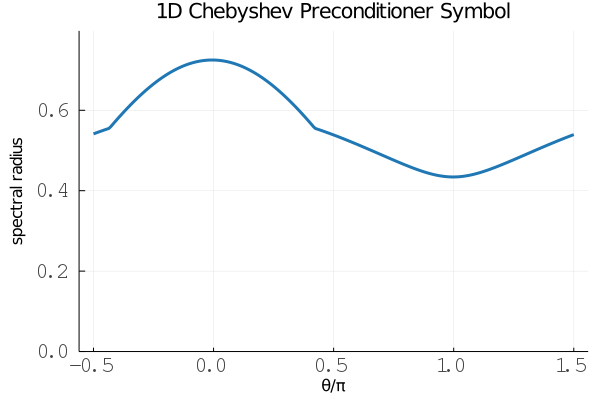
\includegraphics[height=3.9cm]{../img/ChebyshevSymbol1D}
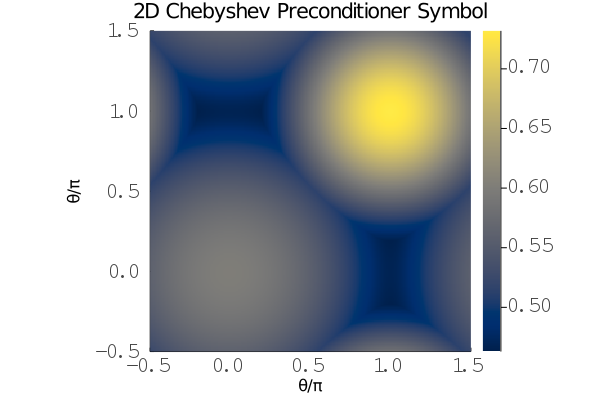
\includegraphics[height=3.9cm]{../img/ChebyshevSymbol2D}

Third order Chebyshev smoothing quartic elements

~\\

low frequencies - $\theta \in T^{\text{low}} = \left[ - \pi / 2, \pi / 2 \right)^d$\\

high frequencies - $\theta \in T^{\text{high}} = \left[ - \pi / 2, 3 \pi / 2 \right)^d \setminus T^{\text{low}}$

\end{center}
\end{frame}

%------------------------------------------------
\section{LFA of Multigrid Methods}
%------------------------------------------------

\begin{frame}
\begin{center}
\frametitle{Two-Grid Multigrid Error}

Multigrid methods target the low frequency error\\

\begin{equation}
\mathbf{E}_{\text{2MG}} = {\color{burgundy}\mathbf{S}}_f \left( \mathbf{I} - {\color{burgundy}\mathbf{P}}_{\text{ctof}} {\color{burgundy}\mathbf{A}}_c^{-1} {\color{burgundy}\mathbf{R}}_{\text{ftoc}} {\color{burgundy}\mathbf{A}}_f \right) {\color{burgundy}\mathbf{S}}_f
\end{equation}

\begin{itemize}

\item ${\color{burgundy}\mathbf{A}}_f$ - fine grid PDE operator

\item ${\color{burgundy}\mathbf{A}}_c^{-1}$ - coarse grid solve (low frequency error)

\item ${\color{burgundy}\mathbf{S}}_f$ - fine grid smoother (high frequency error)

\item ${\color{burgundy}\mathbf{P}}_{\text{ctof}}$ - coarse to fine grid prolongation operator

\item ${\color{burgundy}\mathbf{R}}_{\text{ftoc}}$ - fine to coarse grid restriction operator

\end{itemize}

~\\

Grid transfer operators and coarse representation differentiate h-multigrid and p-multigrid

\end{center}
\end{frame}

%------------------------------------------------

\begin{frame}
\begin{center}
\frametitle{Two-Grid Multigrid Error}

The definition of the symbol follows naturally\\

\begin{equation}
\tilde{\mathbf{E}}_{\text{2MG}} \left( \boldsymbol{\theta} \right) = \tilde{{\color{burgundy}\mathbf{S}}}_f \left( \boldsymbol{\theta}, \omega \right) \left( \mathbf{I} - \tilde{{\color{burgundy}\mathbf{P}}}_{\text{ctof}} \left( \boldsymbol{\theta} \right) \left(\tilde{{\color{burgundy}\mathbf{A}}}_c \left( \boldsymbol{\theta} \right) \right)^{-1} \tilde{{\color{burgundy}\mathbf{R}}}_{\text{ftoc}} \left( \boldsymbol{\theta} \right) \tilde{{\color{burgundy}\mathbf{A}}}_f \left( \boldsymbol{\theta} \right) \right) \tilde{{\color{burgundy}\mathbf{S}}}_f \left( \boldsymbol{\theta}, \omega \right)
\end{equation}

\begin{itemize}

\item ${\color{burgundy}\mathbf{A}}_f$ - fine grid PDE operator

\item ${\color{burgundy}\mathbf{A}}_c^{-1}$ - coarse grid solve (low frequency error)

\item ${\color{burgundy}\mathbf{S}}_f$ - fine grid smoother (high frequency error)

\item ${\color{burgundy}\mathbf{P}}_{\text{ctof}}$ - coarse to fine grid prolongation operator

\item ${\color{burgundy}\mathbf{R}}_{\text{ftoc}}$ - fine to coarse grid restriction operator

\end{itemize}

\end{center}
\end{frame}

%------------------------------------------------

\subsection{P-Multigrid}

\begin{frame}
\begin{center}
\frametitle{P-Multigrid Transfer Operators}

P-multigrid prolongation can be represented as an interpolation\\from the coarse to fine grid\\

\begin{columns}[onlytextwidth]
  \begin{column}{0.45\textwidth}
   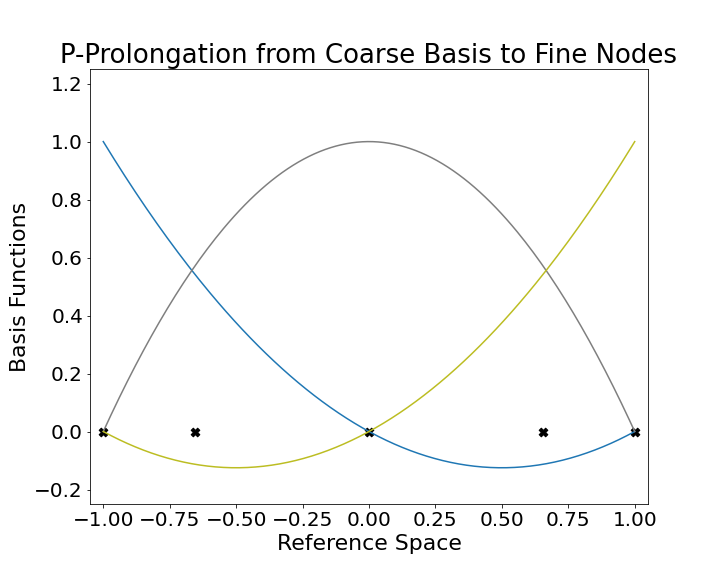
\includegraphics[width=1.0\textwidth]{../img/pProlongation}
  \end{column}

  \begin{column}{0.45\textwidth}
  \begin{equation}
  \begin{gathered}
  {\color{burgundy}\mathbf{P}}_{\text{ctof}} = \mathbf{P}_f^T \mathbf{G}_f^T {\color{burgundy}\mathbf{P}}_e \mathbf{G}_c \mathbf{P}_c\\
  {\color{burgundy}\mathbf{P}}_e = {\color{blue(ncs)}\mathbf{I}} {\color{applegreen}\mathbf{D}}_{\text{scale}} {\color{blue(ncs)}\mathbf{B}}_{\text{ctof}}
  \end{gathered}
  \end{equation}

  $\color{applegreen}\mathbf{D}$ scales for node multiplicity
  \end{column}
\end{columns}

\end{center}
\end{frame}

%------------------------------------------------

\begin{frame}
\begin{center}
\frametitle{Example: P-Multigrid}

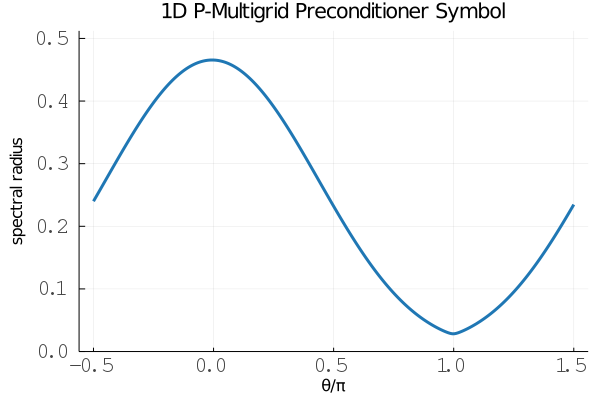
\includegraphics[height=3.9cm]{../img/pmultigridSymbol1D}
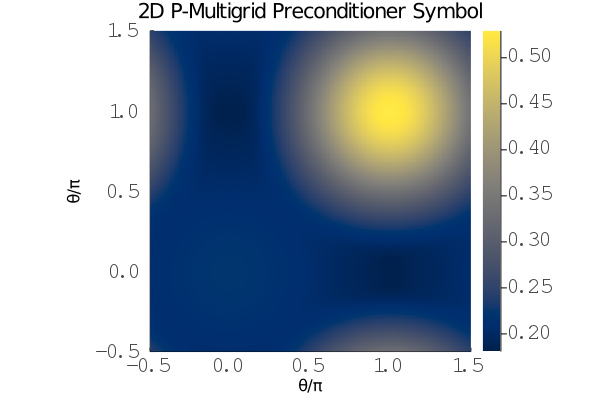
\includegraphics[height=3.9cm]{../img/pmultigridSymbol2D}

p-multigrid with third order Chebyshev on quadratic to linear elements\\

~\\

low frequencies - $\theta \in T^{\text{low}} = \left[ - \pi / 2, \pi / 2 \right)^d$\\

high frequencies - $\theta \in T^{\text{high}} = \left[ - \pi / 2, 3 \pi / 2 \right)^d \setminus T^{\text{low}}$

\end{center}
\end{frame}

%------------------------------------------------

\begin{frame}
\begin{center}
\frametitle{Validation: P-Multigrid}

\begin{table}[ht!]
\begin{center}
\begin{tabular}{l c c}
  \toprule
  $p_{\text{fine}}$ to $p_{\text{coarse}}$  &  LFA  &  libCEED  \\
  %\cmidrule(lr){2-3} \cmidrule(lr){4-5} \cmidrule(lr){6-7}
  \toprule
  $p = 2$ to $p = 1$   &  0.312  &  0.301  \\
  \midrule
  $p = 4$ to $p = 2$   &  1.436  &  1.402  \\
  $p = 4$ to $p = 1$   &  1.436  &  1.401  \\
  \midrule
  $p = 8$ to $p = 4$   &  1.989  &  1.885  \\
  $p = 8$ to $p = 2$   &  1.989  &  1.874  \\
  $p = 8$ to $p = 1$   &  1.989  &  1.875  \\
  \bottomrule
\end{tabular}
\end{center}
\label{table:two_grid_3d_jacobi}
\end{table}

LFA and experimental two-grid convergence factors with Jacobi smoothing for 3D Laplacian with $\omega = 1.0$\\

~\\

3D manufactured solution on the domain $\left[ -3, 3 \right]^3$ with Dirichlet boundaries:

\begin{equation}
f \left( x, y, z \right) = x y z \sin \left( \pi x \right) \sin \left( \pi \left( 1.23 + 0.5 y \right) \right) \sin \left( \pi \left( 2.34 + 0.25 z \right) \right)
\end{equation}

\end{center}
\end{frame}

%------------------------------------------------

\begin{frame}
\begin{center}
\frametitle{Validation: P-Multigrid}

\begin{table}[ht!]
\begin{center}
\begin{tabular}{l cc cc cc}
  \toprule
  $p_{\text{fine}}$ to $p_{\text{coarse}}$  &  \multicolumn{2}{c}{$k = 2$}  &  \multicolumn{2}{c}{$k = 3$}  &  \multicolumn{2}{c}{$k = 4$}  \\
  %\cmidrule(lr){2-3} \cmidrule(lr){4-5} \cmidrule(lr){6-7}
                      &  LFA  &  libCEED  &  LFA  &  libCEED  &  LFA  &  libCEED  \\
  \toprule
  $p = 2$ to $p = 1$  &  0.253 & 0.222  &  0.076 & 0.058  &  0.041 & 0.033  \\
  \midrule
  $p = 4$ to $p = 2$  &  0.277 & 0.251  &  0.111 & 0.097  &  0.062 & 0.050  \\
  $p = 4$ to $p = 1$  &  0.601 & 0.587  &  0.416 & 0.398  &  0.295 & 0.276  \\
  \midrule
  $p = 8$ to $p = 4$  &  0.398 & 0.391  &  0.197 & 0.195  &  0.121 & 0.110  \\
  $p = 8$ to $p = 2$  &  0.748 & 0.743  &  0.611 & 0.603  &  0.506 & 0.469  \\
  $p = 8$ to $p = 1$  &  0.920 & 0.914  &  0.871 & 0.861  &  0.827 & 0.814  \\
  \bottomrule
\end{tabular}
\end{center}
\label{table:two_grid_3d_chebyshev}
\end{table}

LFA and experimental two-grid convergence factors with Chebyshev smoothing for 3D Laplacian\\

\end{center}
\end{frame}

%------------------------------------------------

\subsection{H-Multigrid}

\begin{frame}
\begin{center}
\frametitle{H-Multigrid Transfer Operators}

H-multigrid prolongation can be represented as an interpolation\\from the coarse grid to fine grid macro-elements\\

\begin{columns}[onlytextwidth]
  \begin{column}{0.45\textwidth}
   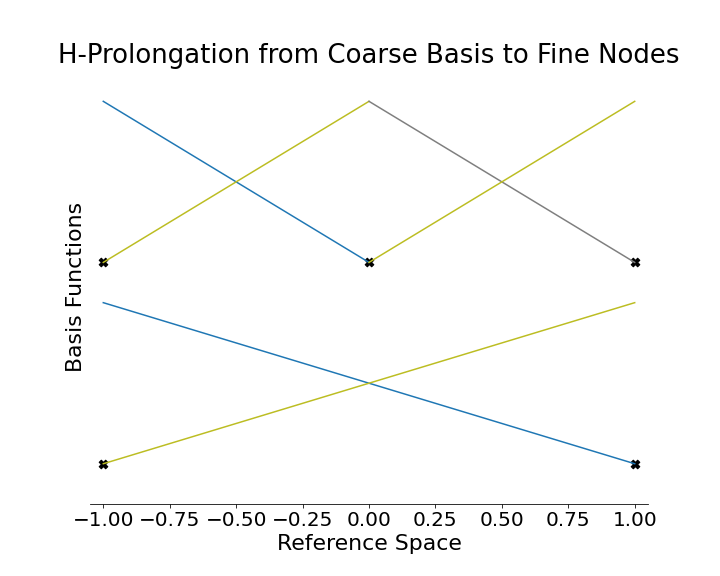
\includegraphics[width=1.0\textwidth]{../img/hProlongation}
  \end{column}

  \begin{column}{0.45\textwidth}
  \begin{equation}
  \begin{gathered}
  {\color{burgundy}\mathbf{P}}_{\text{ctof}} = \mathbf{P}_f^T \mathbf{G}_f^T {\color{burgundy}\mathbf{P}}_e \mathbf{G}_c \mathbf{P}_c\\
  {\color{burgundy}\mathbf{P}}_e = {\color{blue(ncs)}\mathbf{I}} {\color{applegreen}\mathbf{D}}_{\text{scale}} {\color{blue(ncs)}\mathbf{B}}_{\text{ctof}}
  \end{gathered}
  \end{equation}

  $\color{applegreen}\mathbf{D}$ scales for node multiplicity
  \end{column}
\end{columns}

\end{center}
\end{frame}

%------------------------------------------------

\begin{frame}
\begin{center}
\frametitle{Example: H-Multigrid}

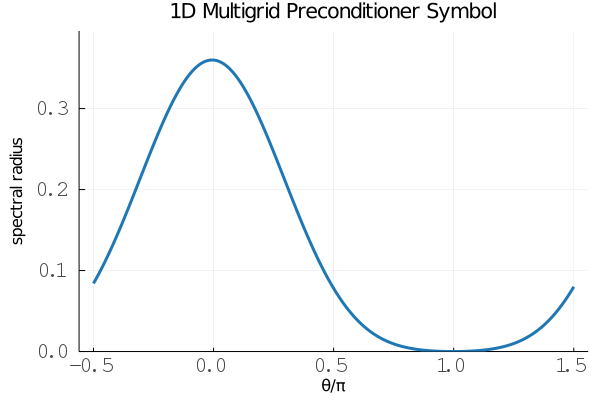
\includegraphics[height=3.9cm]{../img/hmultigridSymbol1D}
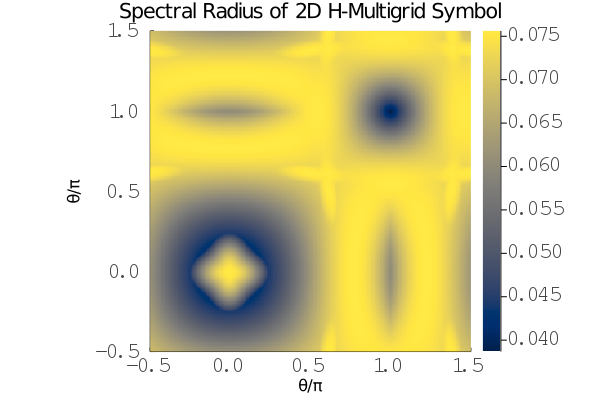
\includegraphics[height=3.9cm]{../img/hmultigridSymbol2D}

h-multigrid with third order Chebyshev on linear elements\\

~\\

low frequencies - $\theta \in T^{\text{low}} = \left[ - \pi / 2, \pi / 2 \right)^d$\\

high frequencies - $\theta \in T^{\text{high}} = \left[ - \pi / 2, 3 \pi / 2 \right)^d \setminus T^{\text{low}}$

\end{center}
\end{frame}

%------------------------------------------------

\begin{frame}
\begin{center}
\frametitle{Validation: P-Multigrid}

\begin{table}[ht!]
\begin{center}
\begin{tabular}{l cc cc cc}
  \toprule
  $p, d$  &  \multicolumn{2}{c}{$\nu = \left( 0, 1 \right)$}  &  \multicolumn{2}{c}{$\nu = \left( 1, 1 \right)$}  &  \multicolumn{2}{c}{$\nu = \left( 2, 2 \right)$}  \\
  %\cmidrule(lr){2-3} \cmidrule(lr){4-5} \cmidrule(lr){6-7}
                      &  $\rho$  &  $\omega$  &  $\rho$ & $\omega$  &  $\rho$ & $\omega$  \\
  \toprule
  $p = 2, d = 1$  &  0.821 & 1.000  &  0.821 & 1.000  &  1.279 & 1.000   \\
  $p = 2, d = 1$  &  0.526 & 0.838  &  0.495 & 0.838  &  0.302 & 0.838   \\
  $p = 2, d = 1$  &  0.291 & 0.709  &  0.249 & 0.709  &  0.064 & 0.709   \\
  \midrule
  $p = 3, d = 1$  &  0.491 & 0.650  &  0.337 & 0.650  &  0.131 & 0.650   \\
  \midrule
  $p = 4, d = 1$  &  0.608 & 0.640  &  0.559 & 0.640  &  0.331 & 0.640   \\
  \midrule
  $p = 2, d = 2$  &  0.452 & 1.000  &  0.288 & 1.000  &  0.091 & 1.000   \\
  \bottomrule
\end{tabular}
\end{center}
\label{table:two_grid_hmultigrid}
\end{table}

Two-grid convergence factor and Jacobi smoothing parameter\\for high-order h-multigrid\\

~\\

Results agree with previous work \cite{he2020two}\\

\end{center}
\end{frame}

%------------------------------------------------
\section{LFA of BDDC}
%------------------------------------------------

\begin{frame}
\begin{center}
\frametitle{Big Picture}

\begin{itemize}

\item High-order matrix-free representations of PDEs are better suited to modern hardware than sparse matrices\\

~\\

\item High-order matrix-free representations require preconditioned iterative solvers\\

~\\

\item Local Fourier Analysis (LFA) provides sharp convergence estimates for these preconditioners\\

~\\

\item We develop LFA of p-multigrid and Balancing Domain Decomposition by Constraints (BDDC) on high-order element subdomains\\

~\\

\item Further, we investigate LFA of p-multigrid with a BDDC smoother

\end{itemize}

\end{center}
\end{frame}

%------------------------------------------------
\section{Summary}
%------------------------------------------------

\begin{frame}
\begin{center}
\frametitle{Big Picture}

\begin{itemize}

\item High-order matrix-free representations of PDEs are better suited to modern hardware than sparse matrices\\

~\\

\item High-order matrix-free representations require preconditioned iterative solvers\\

~\\

\item Local Fourier Analysis (LFA) provides sharp convergence estimates for these preconditioners\\

~\\

\item We develop LFA of p-multigrid and Balancing Domain Decomposition by Constraints (BDDC) on high-order element subdomains\\

~\\

\item Further, we investigate LFA of p-multigrid with a BDDC smoother

\end{itemize}

\end{center}
\end{frame}

%------------------------------------------------

\begin{frame}[noframenumbering]
\titlepage % Print the title page
\end{frame}

\begin{frame}[noframenumbering]
\bibliographystyle{plain}           % or "siam", or "alpha", etc.
\bibliography{../paper/references}  % Bib database in "refs.bib"
\end{frame}

\begin{frame}[noframenumbering]
\titlepage % Print the title page
\end{frame}

%------------------------------------------------

%----------------------------------------------------------------------------------------

\end{document}
